\documentclass[1p]{elsarticle_modified}
%\bibliographystyle{elsarticle-num}

%\usepackage[colorlinks]{hyperref}
%\usepackage{abbrmath_seonhwa} %\Abb, \Ascr, \Acal ,\Abf, \Afrak
\usepackage{amsfonts}
\usepackage{amssymb}
\usepackage{amsmath}
\usepackage{amsthm}
\usepackage{scalefnt}
\usepackage{amsbsy}
\usepackage{kotex}
\usepackage{caption}
\usepackage{subfig}
\usepackage{color}
\usepackage{graphicx}
\usepackage{xcolor} %% white, black, red, green, blue, cyan, magenta, yellow
\usepackage{float}
\usepackage{setspace}
\usepackage{hyperref}

\usepackage{tikz}
\usetikzlibrary{arrows}

\usepackage{multirow}
\usepackage{array} % fixed length table
\usepackage{hhline}

%%%%%%%%%%%%%%%%%%%%%
\makeatletter
\renewcommand*\env@matrix[1][\arraystretch]{%
	\edef\arraystretch{#1}%
	\hskip -\arraycolsep
	\let\@ifnextchar\new@ifnextchar
	\array{*\c@MaxMatrixCols c}}
\makeatother %https://tex.stackexchange.com/questions/14071/how-can-i-increase-the-line-spacing-in-a-matrix
%%%%%%%%%%%%%%%

\usepackage[normalem]{ulem}

\newcommand{\msout}[1]{\ifmmode\text{\sout{\ensuremath{#1}}}\else\sout{#1}\fi}
%SOURCE: \msout is \stkout macro in https://tex.stackexchange.com/questions/20609/strikeout-in-math-mode

\newcommand{\cancel}[1]{
	\ifmmode
	{\color{red}\msout{#1}}
	\else
	{\color{red}\sout{#1}}
	\fi
}

\newcommand{\add}[1]{
	{\color{blue}\uwave{#1}}
}

\newcommand{\replace}[2]{
	\ifmmode
	{\color{red}\msout{#1}}{\color{blue}\uwave{#2}}
	\else
	{\color{red}\sout{#1}}{\color{blue}\uwave{#2}}
	\fi
}

\newcommand{\Sol}{\mathcal{S}} %segment
\newcommand{\D}{D} %diagram
\newcommand{\A}{\mathcal{A}} %arc


%%%%%%%%%%%%%%%%%%%%%%%%%%%%%5 test

\def\sl{\operatorname{\textup{SL}}(2,\Cbb)}
\def\psl{\operatorname{\textup{PSL}}(2,\Cbb)}
\def\quan{\mkern 1mu \triangleright \mkern 1mu}

\theoremstyle{definition}
\newtheorem{thm}{Theorem}[section]
\newtheorem{prop}[thm]{Proposition}
\newtheorem{lem}[thm]{Lemma}
\newtheorem{ques}[thm]{Question}
\newtheorem{cor}[thm]{Corollary}
\newtheorem{defn}[thm]{Definition}
\newtheorem{exam}[thm]{Example}
\newtheorem{rmk}[thm]{Remark}
\newtheorem{alg}[thm]{Algorithm}

\newcommand{\I}{\sqrt{-1}}
\begin{document}

%\begin{frontmatter}
%
%\title{Boundary parabolic representations of knots up to 8 crossings}
%
%%% Group authors per affiliation:
%\author{Yunhi Cho} 
%\address{Department of Mathematics, University of Seoul, Seoul, Korea}
%\ead{yhcho@uos.ac.kr}
%
%
%\author{Seonhwa Kim} %\fnref{s_kim}}
%\address{Center for Geometry and Physics, Institute for Basic Science, Pohang, 37673, Korea}
%\ead{ryeona17@ibs.re.kr}
%
%\author{Hyuk Kim}
%\address{Department of Mathematical Sciences, Seoul National University, Seoul 08826, Korea}
%\ead{hyukkim@snu.ac.kr}
%
%\author{Seokbeom Yoon}
%\address{Department of Mathematical Sciences, Seoul National University, Seoul, 08826,  Korea}
%\ead{sbyoon15@snu.ac.kr}
%
%\begin{abstract}
%We find all boundary parabolic representation of knots up to 8 crossings.
%
%\end{abstract}
%\begin{keyword}
%    \MSC[2010] 57M25 
%\end{keyword}
%
%\end{frontmatter}

%\linenumbers
%\tableofcontents
%
\newcommand\colored[1]{\textcolor{white}{\rule[-0.35ex]{0.8em}{1.4ex}}\kern-0.8em\color{red} #1}%
%\newcommand\colored[1]{\textcolor{white}{ #1}\kern-2.17ex	\textcolor{white}{ #1}\kern-1.81ex	\textcolor{white}{ #1}\kern-2.15ex\color{red}#1	}

{\Large $\underline{12a_{0640}~(K12a_{0640})}$}

\setlength{\tabcolsep}{10pt}
\renewcommand{\arraystretch}{1.6}
\vspace{1cm}\begin{tabular}{m{100pt}>{\centering\arraybackslash}m{274pt}}
\multirow{5}{120pt}{
	\centering
	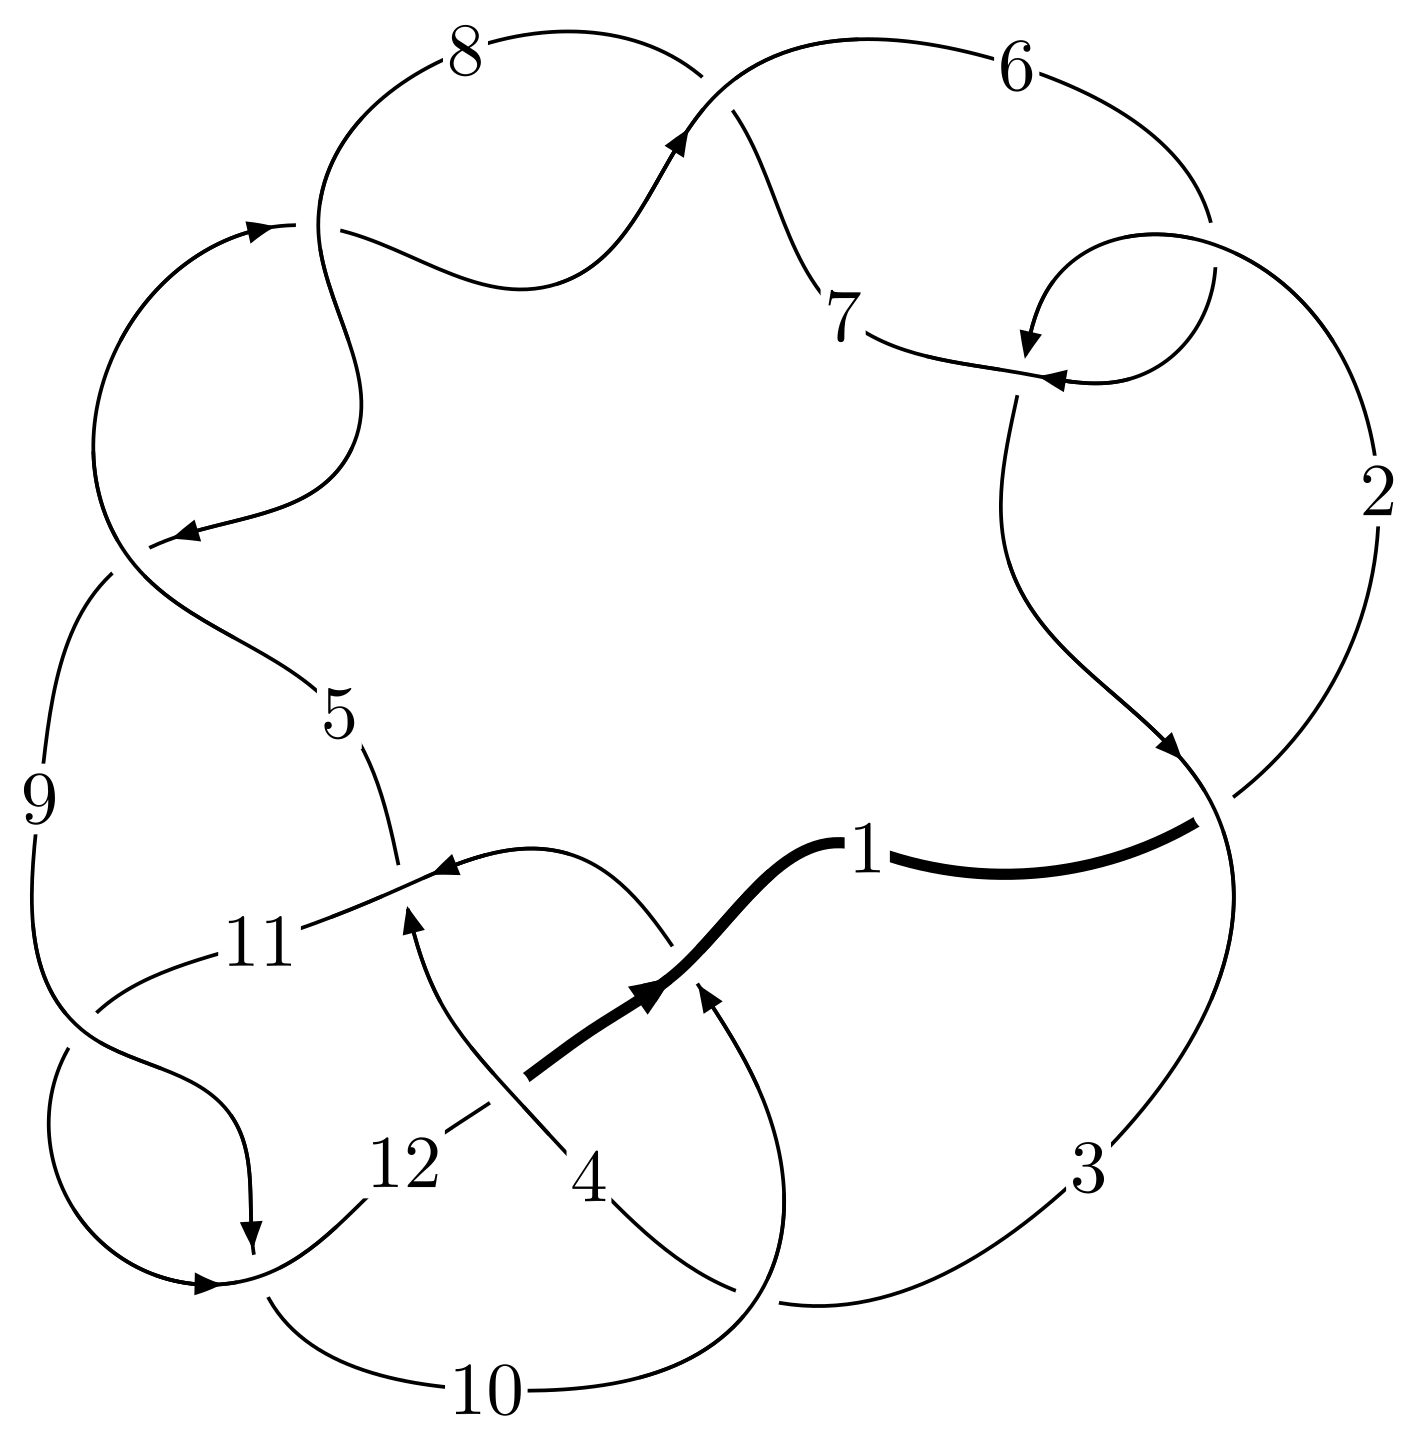
\includegraphics[width=112pt]{../../../GIT/diagram.site/Diagrams/png/1441_12a_0640.png}\\
\ \ \ A knot diagram\footnotemark}&
\allowdisplaybreaks
\textbf{Linearized knot diagam} \\
\cline{2-2}
 &
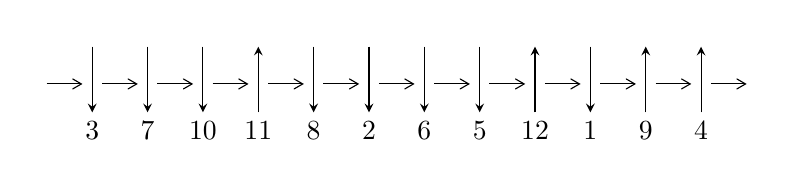
\begin{tikzpicture}[x=20pt, y=17pt]
	% nodes
	\node (C0) at (0, 0) {};
	\node (C1) at (1, 0) {};
	\node (C1U) at (1, +1) {};
	\node (C1D) at (1, -1) {3};

	\node (C2) at (2, 0) {};
	\node (C2U) at (2, +1) {};
	\node (C2D) at (2, -1) {7};

	\node (C3) at (3, 0) {};
	\node (C3U) at (3, +1) {};
	\node (C3D) at (3, -1) {10};

	\node (C4) at (4, 0) {};
	\node (C4U) at (4, +1) {};
	\node (C4D) at (4, -1) {11};

	\node (C5) at (5, 0) {};
	\node (C5U) at (5, +1) {};
	\node (C5D) at (5, -1) {8};

	\node (C6) at (6, 0) {};
	\node (C6U) at (6, +1) {};
	\node (C6D) at (6, -1) {2};

	\node (C7) at (7, 0) {};
	\node (C7U) at (7, +1) {};
	\node (C7D) at (7, -1) {6};

	\node (C8) at (8, 0) {};
	\node (C8U) at (8, +1) {};
	\node (C8D) at (8, -1) {5};

	\node (C9) at (9, 0) {};
	\node (C9U) at (9, +1) {};
	\node (C9D) at (9, -1) {12};

	\node (C10) at (10, 0) {};
	\node (C10U) at (10, +1) {};
	\node (C10D) at (10, -1) {1};

	\node (C11) at (11, 0) {};
	\node (C11U) at (11, +1) {};
	\node (C11D) at (11, -1) {9};

	\node (C12) at (12, 0) {};
	\node (C12U) at (12, +1) {};
	\node (C12D) at (12, -1) {4};
	\node (C13) at (13, 0) {};

	% arrows
	\draw[->,>={angle 60}]
	(C0) edge (C1) (C1) edge (C2) (C2) edge (C3) (C3) edge (C4) (C4) edge (C5) (C5) edge (C6) (C6) edge (C7) (C7) edge (C8) (C8) edge (C9) (C9) edge (C10) (C10) edge (C11) (C11) edge (C12) (C12) edge (C13) ;	\draw[->,>=stealth]
	(C1U) edge (C1D) (C2U) edge (C2D) (C3U) edge (C3D) (C4D) edge (C4U) (C5U) edge (C5D) (C6U) edge (C6D) (C7U) edge (C7D) (C8U) edge (C8D) (C9D) edge (C9U) (C10U) edge (C10D) (C11D) edge (C11U) (C12D) edge (C12U) ;
	\end{tikzpicture} \\
\hhline{~~} \\& 
\textbf{Solving Sequence} \\ \cline{2-2} 
 &
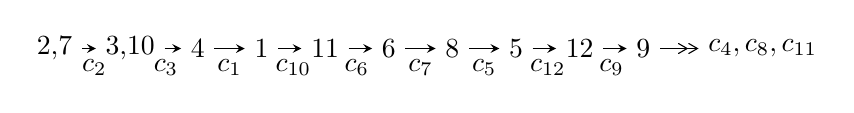
\begin{tikzpicture}[x=23pt, y=7pt]
	% node
	\node (A0) at (-1/8, 0) {2,7};
	\node (A1) at (17/16, 0) {3,10};
	\node (A2) at (17/8, 0) {4};
	\node (A3) at (25/8, 0) {1};
	\node (A4) at (33/8, 0) {11};
	\node (A5) at (41/8, 0) {6};
	\node (A6) at (49/8, 0) {8};
	\node (A7) at (57/8, 0) {5};
	\node (A8) at (65/8, 0) {12};
	\node (A9) at (73/8, 0) {9};
	\node (C1) at (1/2, -1) {$c_{2}$};
	\node (C2) at (13/8, -1) {$c_{3}$};
	\node (C3) at (21/8, -1) {$c_{1}$};
	\node (C4) at (29/8, -1) {$c_{10}$};
	\node (C5) at (37/8, -1) {$c_{6}$};
	\node (C6) at (45/8, -1) {$c_{7}$};
	\node (C7) at (53/8, -1) {$c_{5}$};
	\node (C8) at (61/8, -1) {$c_{12}$};
	\node (C9) at (69/8, -1) {$c_{9}$};
	\node (A10) at (11, 0) {$c_{4},c_{8},c_{11}$};

	% edge
	\draw[->,>=stealth]	
	(A0) edge (A1) (A1) edge (A2) (A2) edge (A3) (A3) edge (A4) (A4) edge (A5) (A5) edge (A6) (A6) edge (A7) (A7) edge (A8) (A8) edge (A9) ;
	\draw[->>,>={angle 60}]	
	(A9) edge (A10);
\end{tikzpicture} \\ 

\end{tabular} \\

\footnotetext{
The image of knot diagram is generated by the software ``\textbf{Draw programme}" developed by Andrew Bartholomew(\url{http://www.layer8.co.uk/maths/draw/index.htm\#Running-draw}), where we modified some parts for our purpose(\url{https://github.com/CATsTAILs/LinksPainter}).
}\phantom \\ \newline 
\centering \textbf{Ideals for irreducible components\footnotemark of $X_{\text{par}}$} 
 
\begin{align*}
I^u_{1}&=\langle 
-1.25642\times10^{19} u^{64}-2.04945\times10^{19} u^{63}+\cdots+2.31572\times10^{19} b-3.37503\times10^{19},\\
\phantom{I^u_{1}}&\phantom{= \langle  }3.33691\times10^{20} u^{64}+8.52592\times10^{20} u^{63}+\cdots+1.62101\times10^{20} a+6.63020\times10^{20},\;u^{65}+2 u^{64}+\cdots-3 u-1\rangle \\
I^u_{2}&=\langle 
b-1,\;u^2+a+u,\;u^3+u^2-1\rangle \\
\\
\end{align*}
\raggedright * 2 irreducible components of $\dim_{\mathbb{C}}=0$, with total 68 representations.\\
\footnotetext{All coefficients of polynomials are rational numbers. But the coefficients are sometimes approximated in decimal forms when there is not enough margin.}
\newpage
\renewcommand{\arraystretch}{1}
\centering \section*{I. $I^u_{1}= \langle -1.26\times10^{19} u^{64}-2.05\times10^{19} u^{63}+\cdots+2.32\times10^{19} b-3.38\times10^{19},\;3.34\times10^{20} u^{64}+8.53\times10^{20} u^{63}+\cdots+1.62\times10^{20} a+6.63\times10^{20},\;u^{65}+2 u^{64}+\cdots-3 u-1 \rangle$}
\flushleft \textbf{(i) Arc colorings}\\
\begin{tabular}{m{7pt} m{180pt} m{7pt} m{180pt} }
\flushright $a_{2}=$&$\begin{pmatrix}1\\0\end{pmatrix}$ \\
\flushright $a_{7}=$&$\begin{pmatrix}0\\u\end{pmatrix}$ \\
\flushright $a_{3}=$&$\begin{pmatrix}1\\u^2\end{pmatrix}$ \\
\flushright $a_{10}=$&$\begin{pmatrix}-2.05854 u^{64}-5.25965 u^{63}+\cdots-6.06473 u-4.09018\\0.542560 u^{64}+0.885015 u^{63}+\cdots+6.46360 u+1.45744\end{pmatrix}$ \\
\flushright $a_{4}=$&$\begin{pmatrix}-4.79404 u^{64}-9.62296 u^{63}+\cdots-15.4240 u-0.688537\\0.228872 u^{64}+3.24003 u^{63}+\cdots+15.0884 u+3.99997\end{pmatrix}$ \\
\flushright $a_{1}=$&$\begin{pmatrix}- u^2+1\\- u^4\end{pmatrix}$ \\
\flushright $a_{11}=$&$\begin{pmatrix}-2.02908 u^{64}-5.22916 u^{63}+\cdots-8.16807 u-4.20542\\0.571011 u^{64}+0.942649 u^{63}+\cdots+6.49245 u+1.42898\end{pmatrix}$ \\
\flushright $a_{6}=$&$\begin{pmatrix}u\\u\end{pmatrix}$ \\
\flushright $a_{8}=$&$\begin{pmatrix}- u^3\\- u^3+u\end{pmatrix}$ \\
\flushright $a_{5}=$&$\begin{pmatrix}u^5+u\\u^5- u^3+u\end{pmatrix}$ \\
\flushright $a_{12}=$&$\begin{pmatrix}2.19411 u^{64}+5.79390 u^{63}+\cdots+9.22067 u+4.42305\\-0.605690 u^{64}-1.01153 u^{63}+\cdots-5.60577 u-1.39431\end{pmatrix}$ \\
\flushright $a_{9}=$&$\begin{pmatrix}- u^7-2 u^3\\- u^7+u^5-2 u^3+u\end{pmatrix}$\\&\end{tabular}
\flushleft \textbf{(ii) Obstruction class $= -1$}\\~\\
\flushleft \textbf{(iii) Cusp Shapes $= -\frac{528336484950614213199}{162100580461622483569} u^{64}-\frac{1127997666238273519001}{162100580461622483569} u^{63}+\cdots-\frac{1505544510775395115944}{162100580461622483569} u-\frac{463719068585525000616}{162100580461622483569}$}\\~\\
\newpage\renewcommand{\arraystretch}{1}
\flushleft \textbf{(iv) u-Polynomials at the component}\newline \\
\begin{tabular}{m{50pt}|m{274pt}}
Crossings & \hspace{64pt}u-Polynomials at each crossing \\
\hline $$\begin{aligned}c_{1},c_{5},c_{7}\\c_{8}\end{aligned}$$&$\begin{aligned}
&u^{65}+12 u^{64}+\cdots+7 u+1
\end{aligned}$\\
\hline $$\begin{aligned}c_{2},c_{6}\end{aligned}$$&$\begin{aligned}
&u^{65}-2 u^{64}+\cdots-3 u+1
\end{aligned}$\\
\hline $$\begin{aligned}c_{3}\end{aligned}$$&$\begin{aligned}
&u^{65}+3 u^{64}+\cdots-742 u+44
\end{aligned}$\\
\hline $$\begin{aligned}c_{4}\end{aligned}$$&$\begin{aligned}
&u^{65}+u^{64}+\cdots+432488 u+133561
\end{aligned}$\\
\hline $$\begin{aligned}c_{9},c_{11}\end{aligned}$$&$\begin{aligned}
&u^{65}+4 u^{64}+\cdots+24 u+1
\end{aligned}$\\
\hline $$\begin{aligned}c_{10}\end{aligned}$$&$\begin{aligned}
&u^{65}-11 u^{64}+\cdots+20 u-8
\end{aligned}$\\
\hline $$\begin{aligned}c_{12}\end{aligned}$$&$\begin{aligned}
&u^{65}+4 u^{64}+\cdots+u+1
\end{aligned}$\\
\hline
\end{tabular}\\~\\
\newpage\renewcommand{\arraystretch}{1}
\flushleft \textbf{(v) Riley Polynomials at the component}\newline \\
\begin{tabular}{m{50pt}|m{274pt}}
Crossings & \hspace{64pt}Riley Polynomials at each crossing \\
\hline $$\begin{aligned}c_{1},c_{5},c_{7}\\c_{8}\end{aligned}$$&$\begin{aligned}
&y^{65}+84 y^{64}+\cdots-5 y-1
\end{aligned}$\\
\hline $$\begin{aligned}c_{2},c_{6}\end{aligned}$$&$\begin{aligned}
&y^{65}-12 y^{64}+\cdots+7 y-1
\end{aligned}$\\
\hline $$\begin{aligned}c_{3}\end{aligned}$$&$\begin{aligned}
&y^{65}+83 y^{64}+\cdots-100900 y-1936
\end{aligned}$\\
\hline $$\begin{aligned}c_{4}\end{aligned}$$&$\begin{aligned}
&y^{65}+19 y^{64}+\cdots+435178968530 y-17838540721
\end{aligned}$\\
\hline $$\begin{aligned}c_{9},c_{11}\end{aligned}$$&$\begin{aligned}
&y^{65}-54 y^{64}+\cdots+1032 y-1
\end{aligned}$\\
\hline $$\begin{aligned}c_{10}\end{aligned}$$&$\begin{aligned}
&y^{65}+21 y^{64}+\cdots+464 y-64
\end{aligned}$\\
\hline $$\begin{aligned}c_{12}\end{aligned}$$&$\begin{aligned}
&y^{65}-8 y^{64}+\cdots+7 y-1
\end{aligned}$\\
\hline
\end{tabular}\\~\\
\newpage\flushleft \textbf{(vi) Complex Volumes and Cusp Shapes}
$$\begin{array}{c|c|c}  
\text{Solutions to }I^u_{1}& \I (\text{vol} + \sqrt{-1}CS) & \text{Cusp shape}\\
 \hline 
\begin{aligned}
u &= -0.820055 + 0.571414 I \\
a &= -0.75883 - 1.23938 I \\
b &= -0.689094 - 0.473723 I\end{aligned}
 & \phantom{-}1.92122 + 2.92849 I & -1.28212 - 3.41898 I \\ \hline\begin{aligned}
u &= -0.820055 - 0.571414 I \\
a &= -0.75883 + 1.23938 I \\
b &= -0.689094 + 0.473723 I\end{aligned}
 & \phantom{-}1.92122 - 2.92849 I & -1.28212 + 3.41898 I \\ \hline\begin{aligned}
u &= -0.969463 + 0.241716 I \\
a &= -1.47695 - 0.01532 I \\
b &= -0.541831 - 0.359416 I\end{aligned}
 & \phantom{-}1.53983 + 7.60011 I & -3.30399 - 8.68829 I \\ \hline\begin{aligned}
u &= -0.969463 - 0.241716 I \\
a &= -1.47695 + 0.01532 I \\
b &= -0.541831 + 0.359416 I\end{aligned}
 & \phantom{-}1.53983 - 7.60011 I & -3.30399 + 8.68829 I \\ \hline\begin{aligned}
u &= \phantom{-}0.744354 + 0.673066 I \\
a &= -1.77437 + 1.77616 I \\
b &= -2.00526 - 0.95542 I\end{aligned}
 & \phantom{-}6.17006 - 0.54961 I & \phantom{-}7.09242 + 0. I\phantom{ +0.000000I} \\ \hline\begin{aligned}
u &= \phantom{-}0.744354 - 0.673066 I \\
a &= -1.77437 - 1.77616 I \\
b &= -2.00526 + 0.95542 I\end{aligned}
 & \phantom{-}6.17006 + 0.54961 I & \phantom{-}7.09242 + 0. I\phantom{ +0.000000I} \\ \hline\begin{aligned}
u &= \phantom{-}0.596268 + 0.796205 I \\
a &= -0.84320 + 1.39289 I \\
b &= -1.84547 + 0.11090 I\end{aligned}
 & \phantom{-}7.82451 + 7.18297 I & \phantom{-}3.58934 - 3.88549 I \\ \hline\begin{aligned}
u &= \phantom{-}0.596268 - 0.796205 I \\
a &= -0.84320 - 1.39289 I \\
b &= -1.84547 - 0.11090 I\end{aligned}
 & \phantom{-}7.82451 - 7.18297 I & \phantom{-}3.58934 + 3.88549 I \\ \hline\begin{aligned}
u &= -0.558053 + 0.817613 I \\
a &= -0.294812 + 1.037710 I \\
b &= \phantom{-}0.840197 + 0.843216 I\end{aligned}
 & \phantom{-}7.30694 + 1.58876 I & \phantom{-}6.94400 - 2.45858 I \\ \hline\begin{aligned}
u &= -0.558053 - 0.817613 I \\
a &= -0.294812 - 1.037710 I \\
b &= \phantom{-}0.840197 - 0.843216 I\end{aligned}
 & \phantom{-}7.30694 - 1.58876 I & \phantom{-}6.94400 + 2.45858 I\\
 \hline 
 \end{array}$$\newpage$$\begin{array}{c|c|c}  
\text{Solutions to }I^u_{1}& \I (\text{vol} + \sqrt{-1}CS) & \text{Cusp shape}\\
 \hline 
\begin{aligned}
u &= \phantom{-}0.998178 + 0.175665 I \\
a &= \phantom{-}0.203083 + 0.942676 I \\
b &= \phantom{-}0.383549 + 0.157322 I\end{aligned}
 & \phantom{-}1.14078 + 1.78516 I & -1.11805 - 3.43956 I \\ \hline\begin{aligned}
u &= \phantom{-}0.998178 - 0.175665 I \\
a &= \phantom{-}0.203083 - 0.942676 I \\
b &= \phantom{-}0.383549 - 0.157322 I\end{aligned}
 & \phantom{-}1.14078 - 1.78516 I & -1.11805 + 3.43956 I \\ \hline\begin{aligned}
u &= -0.767755 + 0.612962 I \\
a &= \phantom{-}3.39308 + 2.93420 I \\
b &= \phantom{-}3.54263 + 0.73826 I\end{aligned}
 & \phantom{-}3.80285 + 2.31034 I & -25.0391 + 4.5996 I \\ \hline\begin{aligned}
u &= -0.767755 - 0.612962 I \\
a &= \phantom{-}3.39308 - 2.93420 I \\
b &= \phantom{-}3.54263 - 0.73826 I\end{aligned}
 & \phantom{-}3.80285 - 2.31034 I & -25.0391 - 4.5996 I \\ \hline\begin{aligned}
u &= \phantom{-}0.812707 + 0.650110 I \\
a &= \phantom{-}0.19129 + 2.01588 I \\
b &= -2.00190 + 1.46282 I\end{aligned}
 & \phantom{-}5.94798 - 4.38359 I & \phantom{-}6.03810 + 7.34576 I \\ \hline\begin{aligned}
u &= \phantom{-}0.812707 - 0.650110 I \\
a &= \phantom{-}0.19129 - 2.01588 I \\
b &= -2.00190 - 1.46282 I\end{aligned}
 & \phantom{-}5.94798 + 4.38359 I & \phantom{-}6.03810 - 7.34576 I \\ \hline\begin{aligned}
u &= \phantom{-}0.870827 + 0.601767 I \\
a &= \phantom{-}1.54614 - 1.58787 I \\
b &= \phantom{-}1.54992 + 0.15321 I\end{aligned}
 & \phantom{-}1.78299 - 6.95651 I & \phantom{-0.000000 -}0. + 9.98928 I \\ \hline\begin{aligned}
u &= \phantom{-}0.870827 - 0.601767 I \\
a &= \phantom{-}1.54614 + 1.58787 I \\
b &= \phantom{-}1.54992 - 0.15321 I\end{aligned}
 & \phantom{-}1.78299 + 6.95651 I & \phantom{-0.000000 } 0. - 9.98928 I \\ \hline\begin{aligned}
u &= \phantom{-}0.648812 + 0.671920 I \\
a &= \phantom{-}0.167707 - 0.999965 I \\
b &= \phantom{-}1.50126 - 0.72002 I\end{aligned}
 & \phantom{-}2.49850 + 2.18973 I & \phantom{-}1.25971 - 3.64342 I \\ \hline\begin{aligned}
u &= \phantom{-}0.648812 - 0.671920 I \\
a &= \phantom{-}0.167707 + 0.999965 I \\
b &= \phantom{-}1.50126 + 0.72002 I\end{aligned}
 & \phantom{-}2.49850 - 2.18973 I & \phantom{-}1.25971 + 3.64342 I\\
 \hline 
 \end{array}$$\newpage$$\begin{array}{c|c|c}  
\text{Solutions to }I^u_{1}& \I (\text{vol} + \sqrt{-1}CS) & \text{Cusp shape}\\
 \hline 
\begin{aligned}
u &= -0.684737 + 0.604855 I \\
a &= -1.010310 - 0.522879 I \\
b &= -1.022020 - 0.286519 I\end{aligned}
 & \phantom{-}2.35987 + 1.53086 I & \phantom{-}1.14672 - 4.64603 I \\ \hline\begin{aligned}
u &= -0.684737 - 0.604855 I \\
a &= -1.010310 + 0.522879 I \\
b &= -1.022020 + 0.286519 I\end{aligned}
 & \phantom{-}2.35987 - 1.53086 I & \phantom{-}1.14672 + 4.64603 I \\ \hline\begin{aligned}
u &= \phantom{-}0.956434 + 0.623323 I \\
a &= -1.40109 + 1.80097 I \\
b &= -2.02007 + 0.57048 I\end{aligned}
 & \phantom{-}6.62284 - 12.39710 I & \phantom{-0.000000 } 0 \\ \hline\begin{aligned}
u &= \phantom{-}0.956434 - 0.623323 I \\
a &= -1.40109 - 1.80097 I \\
b &= -2.02007 - 0.57048 I\end{aligned}
 & \phantom{-}6.62284 + 12.39710 I & \phantom{-0.000000 } 0 \\ \hline\begin{aligned}
u &= -0.831440 + 0.172732 I \\
a &= \phantom{-}2.04727 - 0.37107 I \\
b &= \phantom{-}0.655355 - 0.212384 I\end{aligned}
 & -2.33387 + 3.36125 I & -9.80190 - 7.73059 I \\ \hline\begin{aligned}
u &= -0.831440 - 0.172732 I \\
a &= \phantom{-}2.04727 + 0.37107 I \\
b &= \phantom{-}0.655355 + 0.212384 I\end{aligned}
 & -2.33387 - 3.36125 I & -9.80190 + 7.73059 I \\ \hline\begin{aligned}
u &= \phantom{-}0.798114 + 0.280411 I \\
a &= \phantom{-}0.172582 - 1.311990 I \\
b &= \phantom{-}0.339896 - 0.283030 I\end{aligned}
 & -1.85279 - 0.67069 I & -10.04650 + 3.48460 I \\ \hline\begin{aligned}
u &= \phantom{-}0.798114 - 0.280411 I \\
a &= \phantom{-}0.172582 + 1.311990 I \\
b &= \phantom{-}0.339896 + 0.283030 I\end{aligned}
 & -1.85279 + 0.67069 I & -10.04650 - 3.48460 I \\ \hline\begin{aligned}
u &= -0.994683 + 0.610182 I \\
a &= \phantom{-}1.168940 + 0.182146 I \\
b &= \phantom{-}1.080470 - 0.508571 I\end{aligned}
 & \phantom{-}5.85453 + 3.65774 I & \phantom{-0.000000 } 0 \\ \hline\begin{aligned}
u &= -0.994683 - 0.610182 I \\
a &= \phantom{-}1.168940 - 0.182146 I \\
b &= \phantom{-}1.080470 + 0.508571 I\end{aligned}
 & \phantom{-}5.85453 - 3.65774 I & \phantom{-0.000000 } 0\\
 \hline 
 \end{array}$$\newpage$$\begin{array}{c|c|c}  
\text{Solutions to }I^u_{1}& \I (\text{vol} + \sqrt{-1}CS) & \text{Cusp shape}\\
 \hline 
\begin{aligned}
u &= -0.886696 + 0.799693 I \\
a &= \phantom{-}0.049918 + 0.520198 I \\
b &= \phantom{-}0.688654 + 0.067457 I\end{aligned}
 & \phantom{-}4.04012 + 2.99291 I & \phantom{-0.000000 } 0 \\ \hline\begin{aligned}
u &= -0.886696 - 0.799693 I \\
a &= \phantom{-}0.049918 - 0.520198 I \\
b &= \phantom{-}0.688654 - 0.067457 I\end{aligned}
 & \phantom{-}4.04012 - 2.99291 I & \phantom{-0.000000 } 0 \\ \hline\begin{aligned}
u &= \phantom{-}0.715886\phantom{ +0.000000I} \\
a &= -0.806878\phantom{ +0.000000I} \\
b &= \phantom{-}0.0728787\phantom{ +0.000000I}\end{aligned}
 & -1.06061\phantom{ +0.000000I} & -9.36050\phantom{ +0.000000I} \\ \hline\begin{aligned}
u &= -0.036225 + 0.711406 I \\
a &= -0.646922 - 1.148690 I \\
b &= -0.293062 - 0.445219 I\end{aligned}
 & \phantom{-}4.70553 - 4.54910 I & \phantom{-}4.84912 + 4.44515 I \\ \hline\begin{aligned}
u &= -0.036225 - 0.711406 I \\
a &= -0.646922 + 1.148690 I \\
b &= -0.293062 + 0.445219 I\end{aligned}
 & \phantom{-}4.70553 + 4.54910 I & \phantom{-}4.84912 - 4.44515 I \\ \hline\begin{aligned}
u &= -0.660304 + 0.263461 I \\
a &= -0.92327 - 2.16146 I \\
b &= -0.65397 - 1.36006 I\end{aligned}
 & \phantom{-}1.59886 + 2.23743 I & -0.09200 - 8.25781 I \\ \hline\begin{aligned}
u &= -0.660304 - 0.263461 I \\
a &= -0.92327 + 2.16146 I \\
b &= -0.65397 + 1.36006 I\end{aligned}
 & \phantom{-}1.59886 - 2.23743 I & -0.09200 + 8.25781 I \\ \hline\begin{aligned}
u &= \phantom{-}0.923672 + 0.910982 I \\
a &= -1.33275 + 0.68563 I \\
b &= -2.27621 - 1.05859 I\end{aligned}
 & \phantom{-}11.31760 - 2.00493 I & \phantom{-0.000000 } 0 \\ \hline\begin{aligned}
u &= \phantom{-}0.923672 - 0.910982 I \\
a &= -1.33275 - 0.68563 I \\
b &= -2.27621 + 1.05859 I\end{aligned}
 & \phantom{-}11.31760 + 2.00493 I & \phantom{-0.000000 } 0 \\ \hline\begin{aligned}
u &= -0.920176 + 0.922248 I \\
a &= \phantom{-}0.437881 + 1.136740 I \\
b &= \phantom{-}2.72886 + 0.25698 I\end{aligned}
 & \phantom{-}11.70890 - 2.29417 I & \phantom{-0.000000 } 0\\
 \hline 
 \end{array}$$\newpage$$\begin{array}{c|c|c}  
\text{Solutions to }I^u_{1}& \I (\text{vol} + \sqrt{-1}CS) & \text{Cusp shape}\\
 \hline 
\begin{aligned}
u &= -0.920176 - 0.922248 I \\
a &= \phantom{-}0.437881 - 1.136740 I \\
b &= \phantom{-}2.72886 - 0.25698 I\end{aligned}
 & \phantom{-}11.70890 + 2.29417 I & \phantom{-0.000000 } 0 \\ \hline\begin{aligned}
u &= \phantom{-}0.948041 + 0.898495 I \\
a &= -0.00686 + 1.89178 I \\
b &= -2.10420 + 1.27127 I\end{aligned}
 & \phantom{-}11.23820 - 4.66383 I & \phantom{-0.000000 } 0 \\ \hline\begin{aligned}
u &= \phantom{-}0.948041 - 0.898495 I \\
a &= -0.00686 - 1.89178 I \\
b &= -2.10420 - 1.27127 I\end{aligned}
 & \phantom{-}11.23820 + 4.66383 I & \phantom{-0.000000 } 0 \\ \hline\begin{aligned}
u &= \phantom{-}0.938818 + 0.910131 I \\
a &= \phantom{-}1.94266 - 3.67219 I \\
b &= \phantom{-}6.37132 - 0.20498 I\end{aligned}
 & \phantom{-}13.25270 - 3.35212 I & \phantom{-0.000000 } 0 \\ \hline\begin{aligned}
u &= \phantom{-}0.938818 - 0.910131 I \\
a &= \phantom{-}1.94266 + 3.67219 I \\
b &= \phantom{-}6.37132 + 0.20498 I\end{aligned}
 & \phantom{-}13.25270 + 3.35212 I & \phantom{-0.000000 } 0 \\ \hline\begin{aligned}
u &= -0.906041 + 0.944348 I \\
a &= -0.96248 - 1.58621 I \\
b &= -3.52611 + 0.26832 I\end{aligned}
 & \phantom{-}17.2883 - 8.5608 I & \phantom{-0.000000 } 0 \\ \hline\begin{aligned}
u &= -0.906041 - 0.944348 I \\
a &= -0.96248 + 1.58621 I \\
b &= -3.52611 - 0.26832 I\end{aligned}
 & \phantom{-}17.2883 + 8.5608 I & \phantom{-0.000000 } 0 \\ \hline\begin{aligned}
u &= \phantom{-}0.902391 + 0.951587 I \\
a &= \phantom{-}0.047768 - 1.069910 I \\
b &= \phantom{-}1.97152 - 0.78996 I\end{aligned}
 & \phantom{-}16.6895 + 0.2053 I & \phantom{-0.000000 } 0 \\ \hline\begin{aligned}
u &= \phantom{-}0.902391 - 0.951587 I \\
a &= \phantom{-}0.047768 + 1.069910 I \\
b &= \phantom{-}1.97152 + 0.78996 I\end{aligned}
 & \phantom{-}16.6895 - 0.2053 I & \phantom{-0.000000 } 0 \\ \hline\begin{aligned}
u &= -0.936676 + 0.920511 I \\
a &= -1.11522 - 1.81897 I \\
b &= -3.01179 + 1.07212 I\end{aligned}
 & \phantom{-}15.9561 + 1.1091 I & \phantom{-0.000000 } 0\\
 \hline 
 \end{array}$$\newpage$$\begin{array}{c|c|c}  
\text{Solutions to }I^u_{1}& \I (\text{vol} + \sqrt{-1}CS) & \text{Cusp shape}\\
 \hline 
\begin{aligned}
u &= -0.936676 - 0.920511 I \\
a &= -1.11522 + 1.81897 I \\
b &= -3.01179 - 1.07212 I\end{aligned}
 & \phantom{-}15.9561 - 1.1091 I & \phantom{-0.000000 } 0 \\ \hline\begin{aligned}
u &= -0.958520 + 0.902088 I \\
a &= \phantom{-}0.73789 + 1.98899 I \\
b &= \phantom{-}2.69761 - 0.07690 I\end{aligned}
 & \phantom{-}11.5836 + 9.0106 I & \phantom{-0.000000 } 0 \\ \hline\begin{aligned}
u &= -0.958520 - 0.902088 I \\
a &= \phantom{-}0.73789 - 1.98899 I \\
b &= \phantom{-}2.69761 + 0.07690 I\end{aligned}
 & \phantom{-}11.5836 - 9.0106 I & \phantom{-0.000000 } 0 \\ \hline\begin{aligned}
u &= -0.948403 + 0.914191 I \\
a &= \phantom{-}0.16245 - 1.67524 I \\
b &= -3.04131 - 1.20975 I\end{aligned}
 & \phantom{-}15.9177 + 5.6422 I & \phantom{-0.000000 } 0 \\ \hline\begin{aligned}
u &= -0.948403 - 0.914191 I \\
a &= \phantom{-}0.16245 + 1.67524 I \\
b &= -3.04131 + 1.20975 I\end{aligned}
 & \phantom{-}15.9177 - 5.6422 I & \phantom{-0.000000 } 0 \\ \hline\begin{aligned}
u &= -0.981573 + 0.901998 I \\
a &= -0.76506 - 2.45787 I \\
b &= -3.56067 - 0.50087 I\end{aligned}
 & \phantom{-}17.0389 + 15.3461 I & \phantom{-0.000000 } 0 \\ \hline\begin{aligned}
u &= -0.981573 - 0.901998 I \\
a &= -0.76506 + 2.45787 I \\
b &= -3.56067 + 0.50087 I\end{aligned}
 & \phantom{-}17.0389 - 15.3461 I & \phantom{-0.000000 } 0 \\ \hline\begin{aligned}
u &= \phantom{-}0.988719 + 0.902991 I \\
a &= \phantom{-}0.98242 - 1.12974 I \\
b &= \phantom{-}2.00991 + 0.63394 I\end{aligned}
 & \phantom{-}16.4045 - 7.0166 I & \phantom{-0.000000 } 0 \\ \hline\begin{aligned}
u &= \phantom{-}0.988719 - 0.902991 I \\
a &= \phantom{-}0.98242 + 1.12974 I \\
b &= \phantom{-}2.00991 - 0.63394 I\end{aligned}
 & \phantom{-}16.4045 + 7.0166 I & \phantom{-0.000000 } 0 \\ \hline\begin{aligned}
u &= \phantom{-}0.656202 + 0.074693 I \\
a &= -0.19941 + 2.76051 I \\
b &= \phantom{-}0.712381 - 1.203220 I\end{aligned}
 & \phantom{-}0.647228 - 0.175412 I & \phantom{-}27.9047 - 7.2168 I\\
 \hline 
 \end{array}$$\newpage$$\begin{array}{c|c|c}  
\text{Solutions to }I^u_{1}& \I (\text{vol} + \sqrt{-1}CS) & \text{Cusp shape}\\
 \hline 
\begin{aligned}
u &= \phantom{-}0.656202 - 0.074693 I \\
a &= -0.19941 - 2.76051 I \\
b &= \phantom{-}0.712381 + 1.203220 I\end{aligned}
 & \phantom{-}0.647228 + 0.175412 I & \phantom{-}27.9047 + 7.2168 I \\ \hline\begin{aligned}
u &= \phantom{-}0.025083 + 0.412212 I \\
a &= -0.276764 + 0.598990 I \\
b &= \phantom{-}0.383965 + 0.619009 I\end{aligned}
 & \phantom{-}0.08844 - 1.51243 I & \phantom{-}0.26581 + 4.27826 I \\ \hline\begin{aligned}
u &= \phantom{-}0.025083 - 0.412212 I \\
a &= -0.276764 - 0.598990 I \\
b &= \phantom{-}0.383965 - 0.619009 I\end{aligned}
 & \phantom{-}0.08844 + 1.51243 I & \phantom{-}0.26581 - 4.27826 I \\ \hline\begin{aligned}
u &= -0.305765 + 0.261881 I \\
a &= -4.05933 - 1.09380 I \\
b &= -0.900970 + 0.336871 I\end{aligned}
 & \phantom{-}2.53402 - 0.11660 I & \phantom{-}3.78096 - 2.55604 I \\ \hline\begin{aligned}
u &= -0.305765 - 0.261881 I \\
a &= -4.05933 + 1.09380 I \\
b &= -0.900970 - 0.336871 I\end{aligned}
 & \phantom{-}2.53402 + 0.11660 I & \phantom{-}3.78096 + 2.55604 I\\
 \hline 
 \end{array}$$\newpage\newpage\renewcommand{\arraystretch}{1}
\centering \section*{II. $I^u_{2}= \langle b-1,\;u^2+a+u,\;u^3+u^2-1 \rangle$}
\flushleft \textbf{(i) Arc colorings}\\
\begin{tabular}{m{7pt} m{180pt} m{7pt} m{180pt} }
\flushright $a_{2}=$&$\begin{pmatrix}1\\0\end{pmatrix}$ \\
\flushright $a_{7}=$&$\begin{pmatrix}0\\u\end{pmatrix}$ \\
\flushright $a_{3}=$&$\begin{pmatrix}1\\u^2\end{pmatrix}$ \\
\flushright $a_{10}=$&$\begin{pmatrix}- u^2- u\\1\end{pmatrix}$ \\
\flushright $a_{4}=$&$\begin{pmatrix}- u^2- u\\u^2+u+1\end{pmatrix}$ \\
\flushright $a_{1}=$&$\begin{pmatrix}- u^2+1\\- u^2- u+1\end{pmatrix}$ \\
\flushright $a_{11}=$&$\begin{pmatrix}- u^2- u\\1\end{pmatrix}$ \\
\flushright $a_{6}=$&$\begin{pmatrix}u\\u\end{pmatrix}$ \\
\flushright $a_{8}=$&$\begin{pmatrix}u^2-1\\u^2+u-1\end{pmatrix}$ \\
\flushright $a_{5}=$&$\begin{pmatrix}1\\u^2\end{pmatrix}$ \\
\flushright $a_{12}=$&$\begin{pmatrix}- u^2- u+1\\1\end{pmatrix}$ \\
\flushright $a_{9}=$&$\begin{pmatrix}-1\\0\end{pmatrix}$\\&\end{tabular}
\flushleft \textbf{(ii) Obstruction class $= 1$}\\~\\
\flushleft \textbf{(iii) Cusp Shapes $= u^2+4$}\\~\\
\newpage\renewcommand{\arraystretch}{1}
\flushleft \textbf{(iv) u-Polynomials at the component}\newline \\
\begin{tabular}{m{50pt}|m{274pt}}
Crossings & \hspace{64pt}u-Polynomials at each crossing \\
\hline $$\begin{aligned}c_{1},c_{5},c_{12}\end{aligned}$$&$\begin{aligned}
&u^3- u^2+2 u-1
\end{aligned}$\\
\hline $$\begin{aligned}c_{2}\end{aligned}$$&$\begin{aligned}
&u^3+u^2-1
\end{aligned}$\\
\hline $$\begin{aligned}c_{3},c_{4}\end{aligned}$$&$\begin{aligned}
&u^3-2 u^2+u-1
\end{aligned}$\\
\hline $$\begin{aligned}c_{6}\end{aligned}$$&$\begin{aligned}
&u^3- u^2+1
\end{aligned}$\\
\hline $$\begin{aligned}c_{7},c_{8}\end{aligned}$$&$\begin{aligned}
&u^3+u^2+2 u+1
\end{aligned}$\\
\hline $$\begin{aligned}c_{9}\end{aligned}$$&$\begin{aligned}
&(u+1)^3
\end{aligned}$\\
\hline $$\begin{aligned}c_{10}\end{aligned}$$&$\begin{aligned}
&u^3
\end{aligned}$\\
\hline $$\begin{aligned}c_{11}\end{aligned}$$&$\begin{aligned}
&(u-1)^3
\end{aligned}$\\
\hline
\end{tabular}\\~\\
\newpage\renewcommand{\arraystretch}{1}
\flushleft \textbf{(v) Riley Polynomials at the component}\newline \\
\begin{tabular}{m{50pt}|m{274pt}}
Crossings & \hspace{64pt}Riley Polynomials at each crossing \\
\hline $$\begin{aligned}c_{1},c_{5},c_{7}\\c_{8},c_{12}\end{aligned}$$&$\begin{aligned}
&y^3+3 y^2+2 y-1
\end{aligned}$\\
\hline $$\begin{aligned}c_{2},c_{6}\end{aligned}$$&$\begin{aligned}
&y^3- y^2+2 y-1
\end{aligned}$\\
\hline $$\begin{aligned}c_{3},c_{4}\end{aligned}$$&$\begin{aligned}
&y^3-2 y^2-3 y-1
\end{aligned}$\\
\hline $$\begin{aligned}c_{9},c_{11}\end{aligned}$$&$\begin{aligned}
&(y-1)^3
\end{aligned}$\\
\hline $$\begin{aligned}c_{10}\end{aligned}$$&$\begin{aligned}
&y^3
\end{aligned}$\\
\hline
\end{tabular}\\~\\
\newpage\flushleft \textbf{(vi) Complex Volumes and Cusp Shapes}
$$\begin{array}{c|c|c}  
\text{Solutions to }I^u_{2}& \I (\text{vol} + \sqrt{-1}CS) & \text{Cusp shape}\\
 \hline 
\begin{aligned}
u &= -0.877439 + 0.744862 I \\
a &= \phantom{-}0.662359 + 0.562280 I \\
b &= \phantom{-}1.00000\phantom{ +0.000000I}\end{aligned}
 & \phantom{-}4.66906 + 2.82812 I & \phantom{-}4.21508 - 1.30714 I \\ \hline\begin{aligned}
u &= -0.877439 - 0.744862 I \\
a &= \phantom{-}0.662359 - 0.562280 I \\
b &= \phantom{-}1.00000\phantom{ +0.000000I}\end{aligned}
 & \phantom{-}4.66906 - 2.82812 I & \phantom{-}4.21508 + 1.30714 I \\ \hline\begin{aligned}
u &= \phantom{-}0.754878\phantom{ +0.000000I} \\
a &= -1.32472\phantom{ +0.000000I} \\
b &= \phantom{-}1.00000\phantom{ +0.000000I}\end{aligned}
 & \phantom{-}0.531480\phantom{ +0.000000I} & \phantom{-}4.56980\phantom{ +0.000000I}\\
 \hline 
 \end{array}$$\newpage
\newpage\renewcommand{\arraystretch}{1}
\centering \section*{ III. u-Polynomials}
\begin{tabular}{m{50pt}|m{274pt}}
Crossings & \hspace{64pt}u-Polynomials at each crossing \\
\hline $$\begin{aligned}c_{1},c_{5}\end{aligned}$$&$\begin{aligned}
&(u^3- u^2+2 u-1)(u^{65}+12 u^{64}+\cdots+7 u+1)
\end{aligned}$\\
\hline $$\begin{aligned}c_{2}\end{aligned}$$&$\begin{aligned}
&(u^3+u^2-1)(u^{65}-2 u^{64}+\cdots-3 u+1)
\end{aligned}$\\
\hline $$\begin{aligned}c_{3}\end{aligned}$$&$\begin{aligned}
&(u^3-2 u^2+u-1)(u^{65}+3 u^{64}+\cdots-742 u+44)
\end{aligned}$\\
\hline $$\begin{aligned}c_{4}\end{aligned}$$&$\begin{aligned}
&(u^3-2 u^2+u-1)(u^{65}+u^{64}+\cdots+432488 u+133561)
\end{aligned}$\\
\hline $$\begin{aligned}c_{6}\end{aligned}$$&$\begin{aligned}
&(u^3- u^2+1)(u^{65}-2 u^{64}+\cdots-3 u+1)
\end{aligned}$\\
\hline $$\begin{aligned}c_{7},c_{8}\end{aligned}$$&$\begin{aligned}
&(u^3+u^2+2 u+1)(u^{65}+12 u^{64}+\cdots+7 u+1)
\end{aligned}$\\
\hline $$\begin{aligned}c_{9}\end{aligned}$$&$\begin{aligned}
&((u+1)^3)(u^{65}+4 u^{64}+\cdots+24 u+1)
\end{aligned}$\\
\hline $$\begin{aligned}c_{10}\end{aligned}$$&$\begin{aligned}
&u^3(u^{65}-11 u^{64}+\cdots+20 u-8)
\end{aligned}$\\
\hline $$\begin{aligned}c_{11}\end{aligned}$$&$\begin{aligned}
&((u-1)^3)(u^{65}+4 u^{64}+\cdots+24 u+1)
\end{aligned}$\\
\hline $$\begin{aligned}c_{12}\end{aligned}$$&$\begin{aligned}
&(u^3- u^2+2 u-1)(u^{65}+4 u^{64}+\cdots+u+1)
\end{aligned}$\\
\hline
\end{tabular}\newpage\renewcommand{\arraystretch}{1}
\centering \section*{ IV. Riley Polynomials}
\begin{tabular}{m{50pt}|m{274pt}}
Crossings & \hspace{64pt}Riley Polynomials at each crossing \\
\hline $$\begin{aligned}c_{1},c_{5},c_{7}\\c_{8}\end{aligned}$$&$\begin{aligned}
&(y^3+3 y^2+2 y-1)(y^{65}+84 y^{64}+\cdots-5 y-1)
\end{aligned}$\\
\hline $$\begin{aligned}c_{2},c_{6}\end{aligned}$$&$\begin{aligned}
&(y^3- y^2+2 y-1)(y^{65}-12 y^{64}+\cdots+7 y-1)
\end{aligned}$\\
\hline $$\begin{aligned}c_{3}\end{aligned}$$&$\begin{aligned}
&(y^3-2 y^2-3 y-1)(y^{65}+83 y^{64}+\cdots-100900 y-1936)
\end{aligned}$\\
\hline $$\begin{aligned}c_{4}\end{aligned}$$&$\begin{aligned}
&(y^3-2 y^2-3 y-1)\\
&\cdot(y^{65}+19 y^{64}+\cdots+435178968530 y-17838540721)
\end{aligned}$\\
\hline $$\begin{aligned}c_{9},c_{11}\end{aligned}$$&$\begin{aligned}
&((y-1)^3)(y^{65}-54 y^{64}+\cdots+1032 y-1)
\end{aligned}$\\
\hline $$\begin{aligned}c_{10}\end{aligned}$$&$\begin{aligned}
&y^3(y^{65}+21 y^{64}+\cdots+464 y-64)
\end{aligned}$\\
\hline $$\begin{aligned}c_{12}\end{aligned}$$&$\begin{aligned}
&(y^3+3 y^2+2 y-1)(y^{65}-8 y^{64}+\cdots+7 y-1)
\end{aligned}$\\
\hline
\end{tabular}
\vskip 2pc
\end{document}